\section{Segundo objetivo - débito}

No segundo objetivo vamos analisar valores de débito para 2 casos distintos.
No primeiro caso iremos considerar $T_{idle} = 1~u.t.$, $T_{succ} = 150~u.t.$
e $T_{coll} = 160~u.t.$, que representa a implementação do IEEE 802.11.
Assim, uma transmissão bem-sucedida irá demorar 
150 vezes mais que um \textit{slot} onde ninguém transmite, e uma colisão irá
demorar 160 vezes mais.

No segundo caso, todos os tempos são iguais: $T_{idle} = T_{succ} = T_{coll}$
(\textit{slotted} ALOHA).

\vspace{\baselineskip}
\begin{figure}[h]
    \centering
    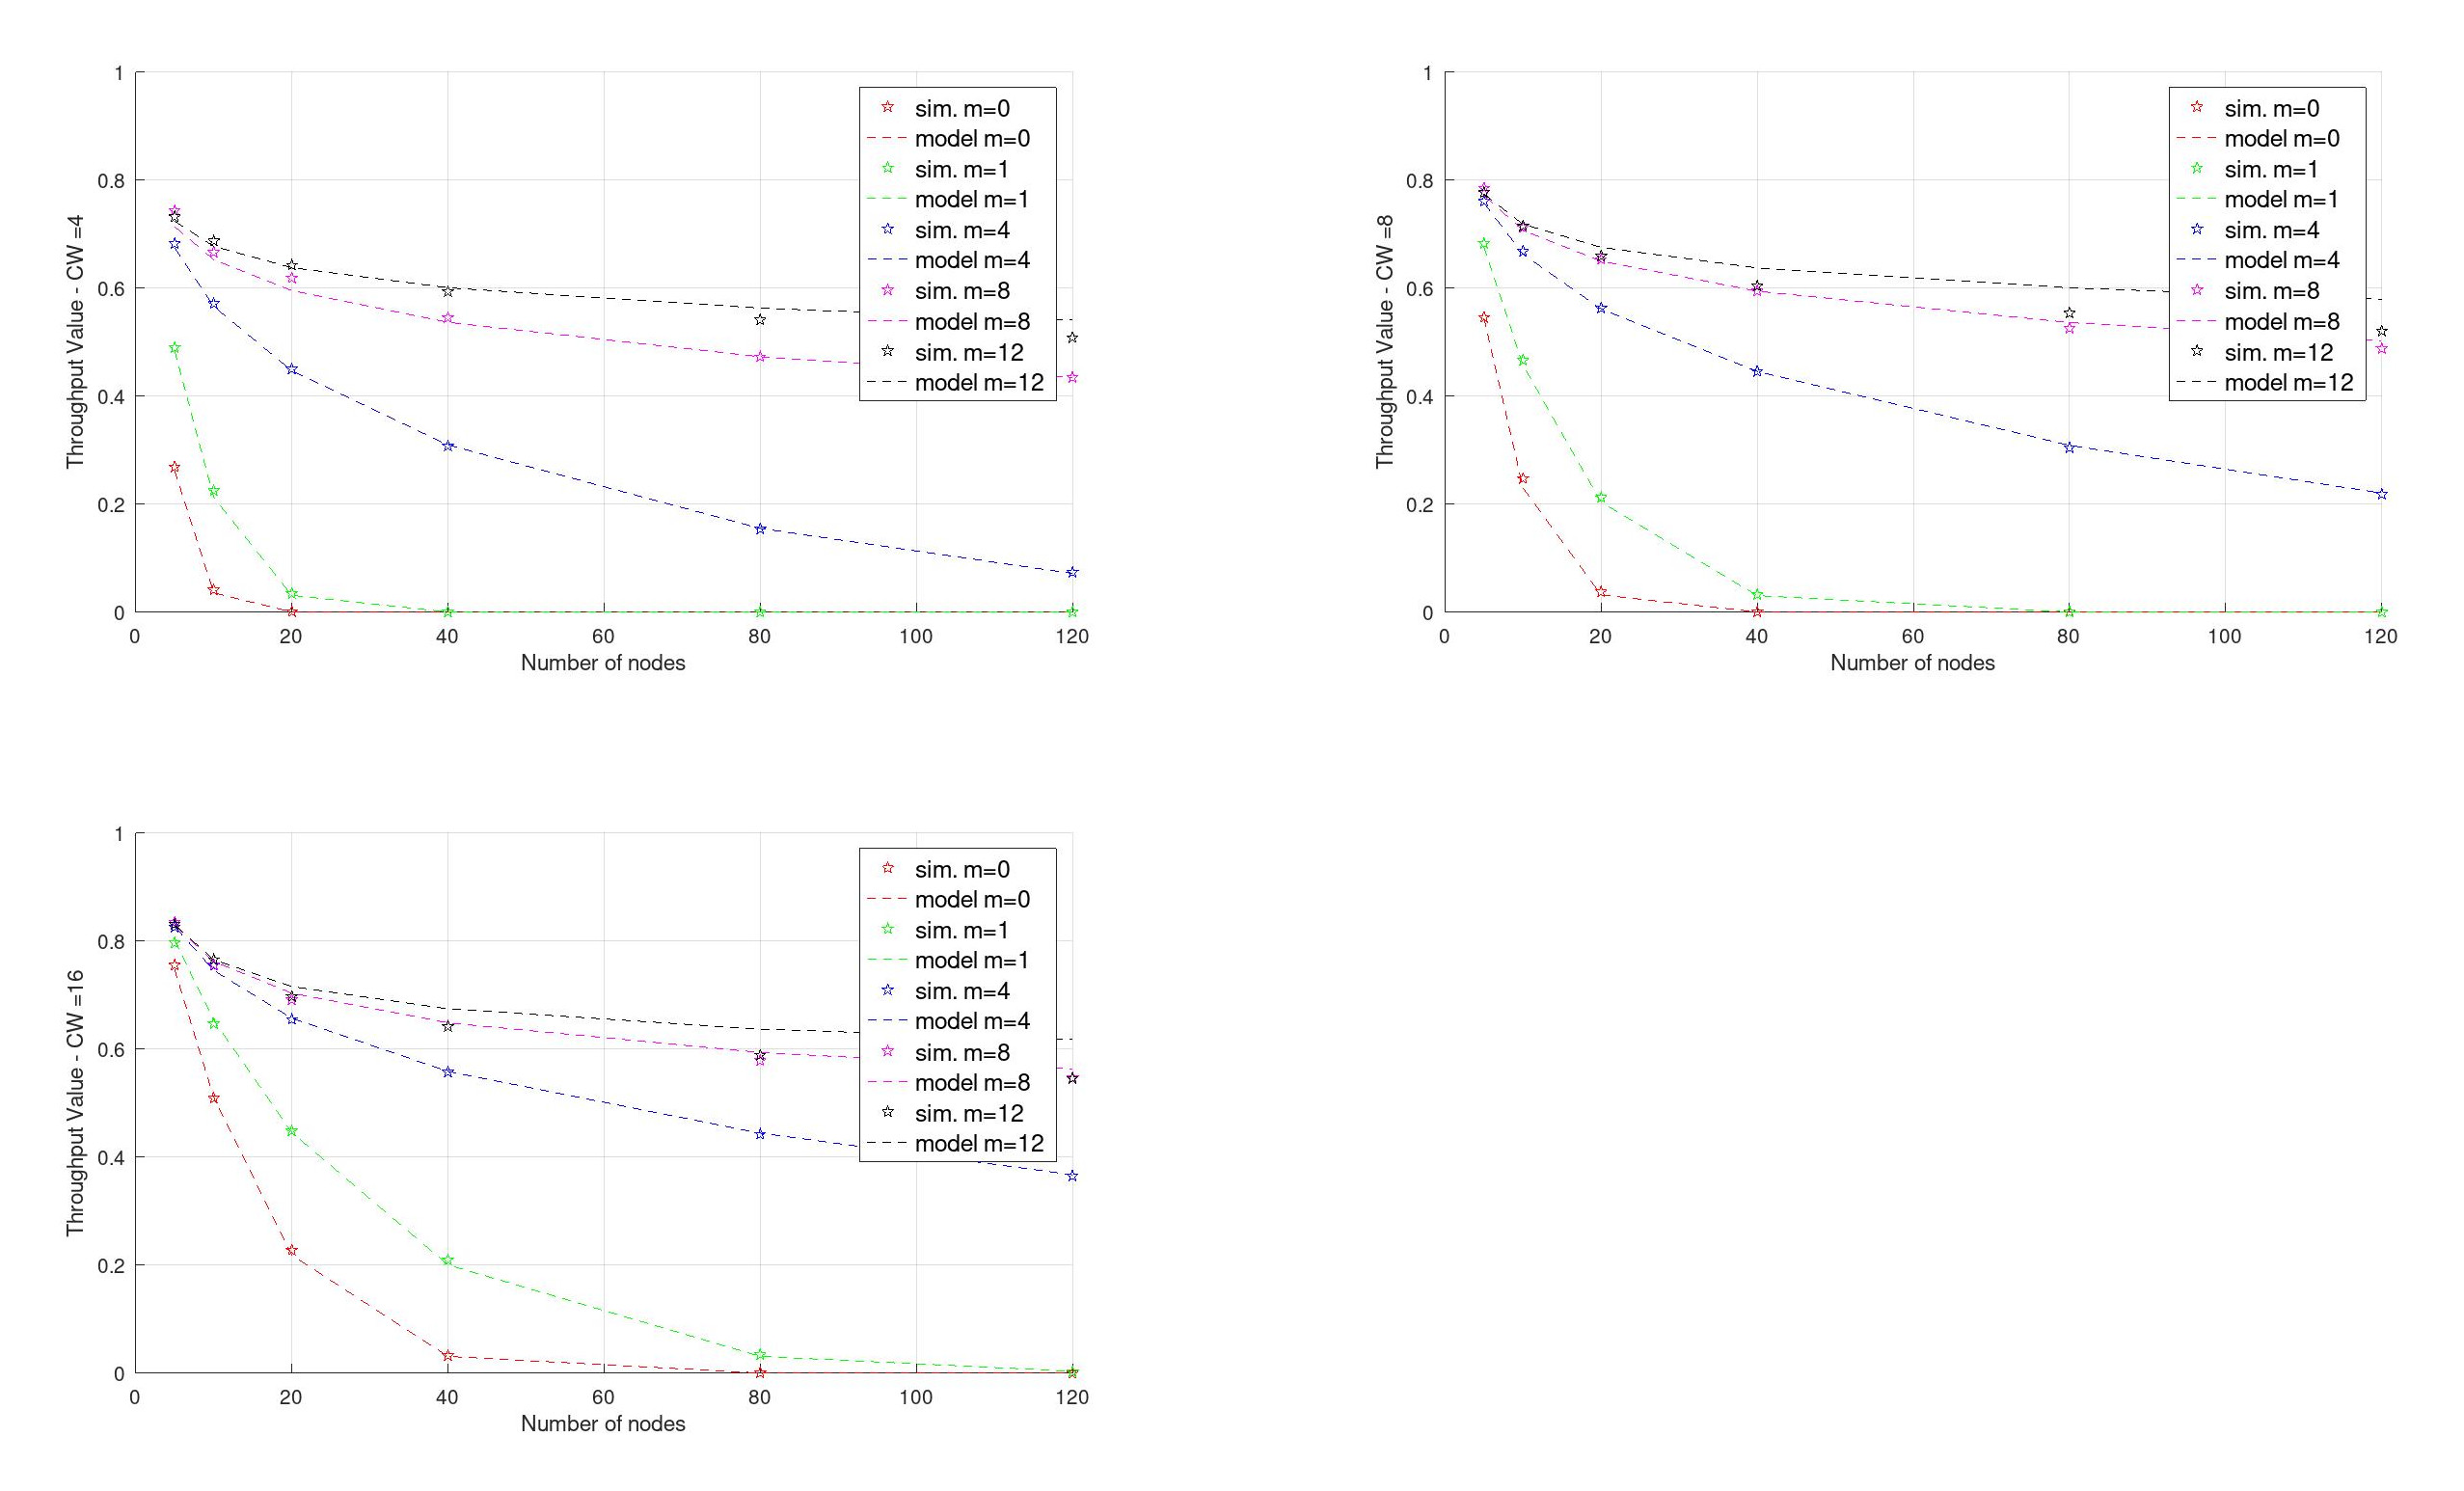
\includegraphics[scale=.18]{Images/objetivo2_1.jpeg}
    \caption{Débito para $T_{succ} = 150~u.t.$ e $T_{coll} = 160~u.t.$}
    \label{fig:objetivo2_1}
\end{figure}
\vspace{\baselineskip}

\vspace{\baselineskip}
\begin{figure}[h]
    \centering
    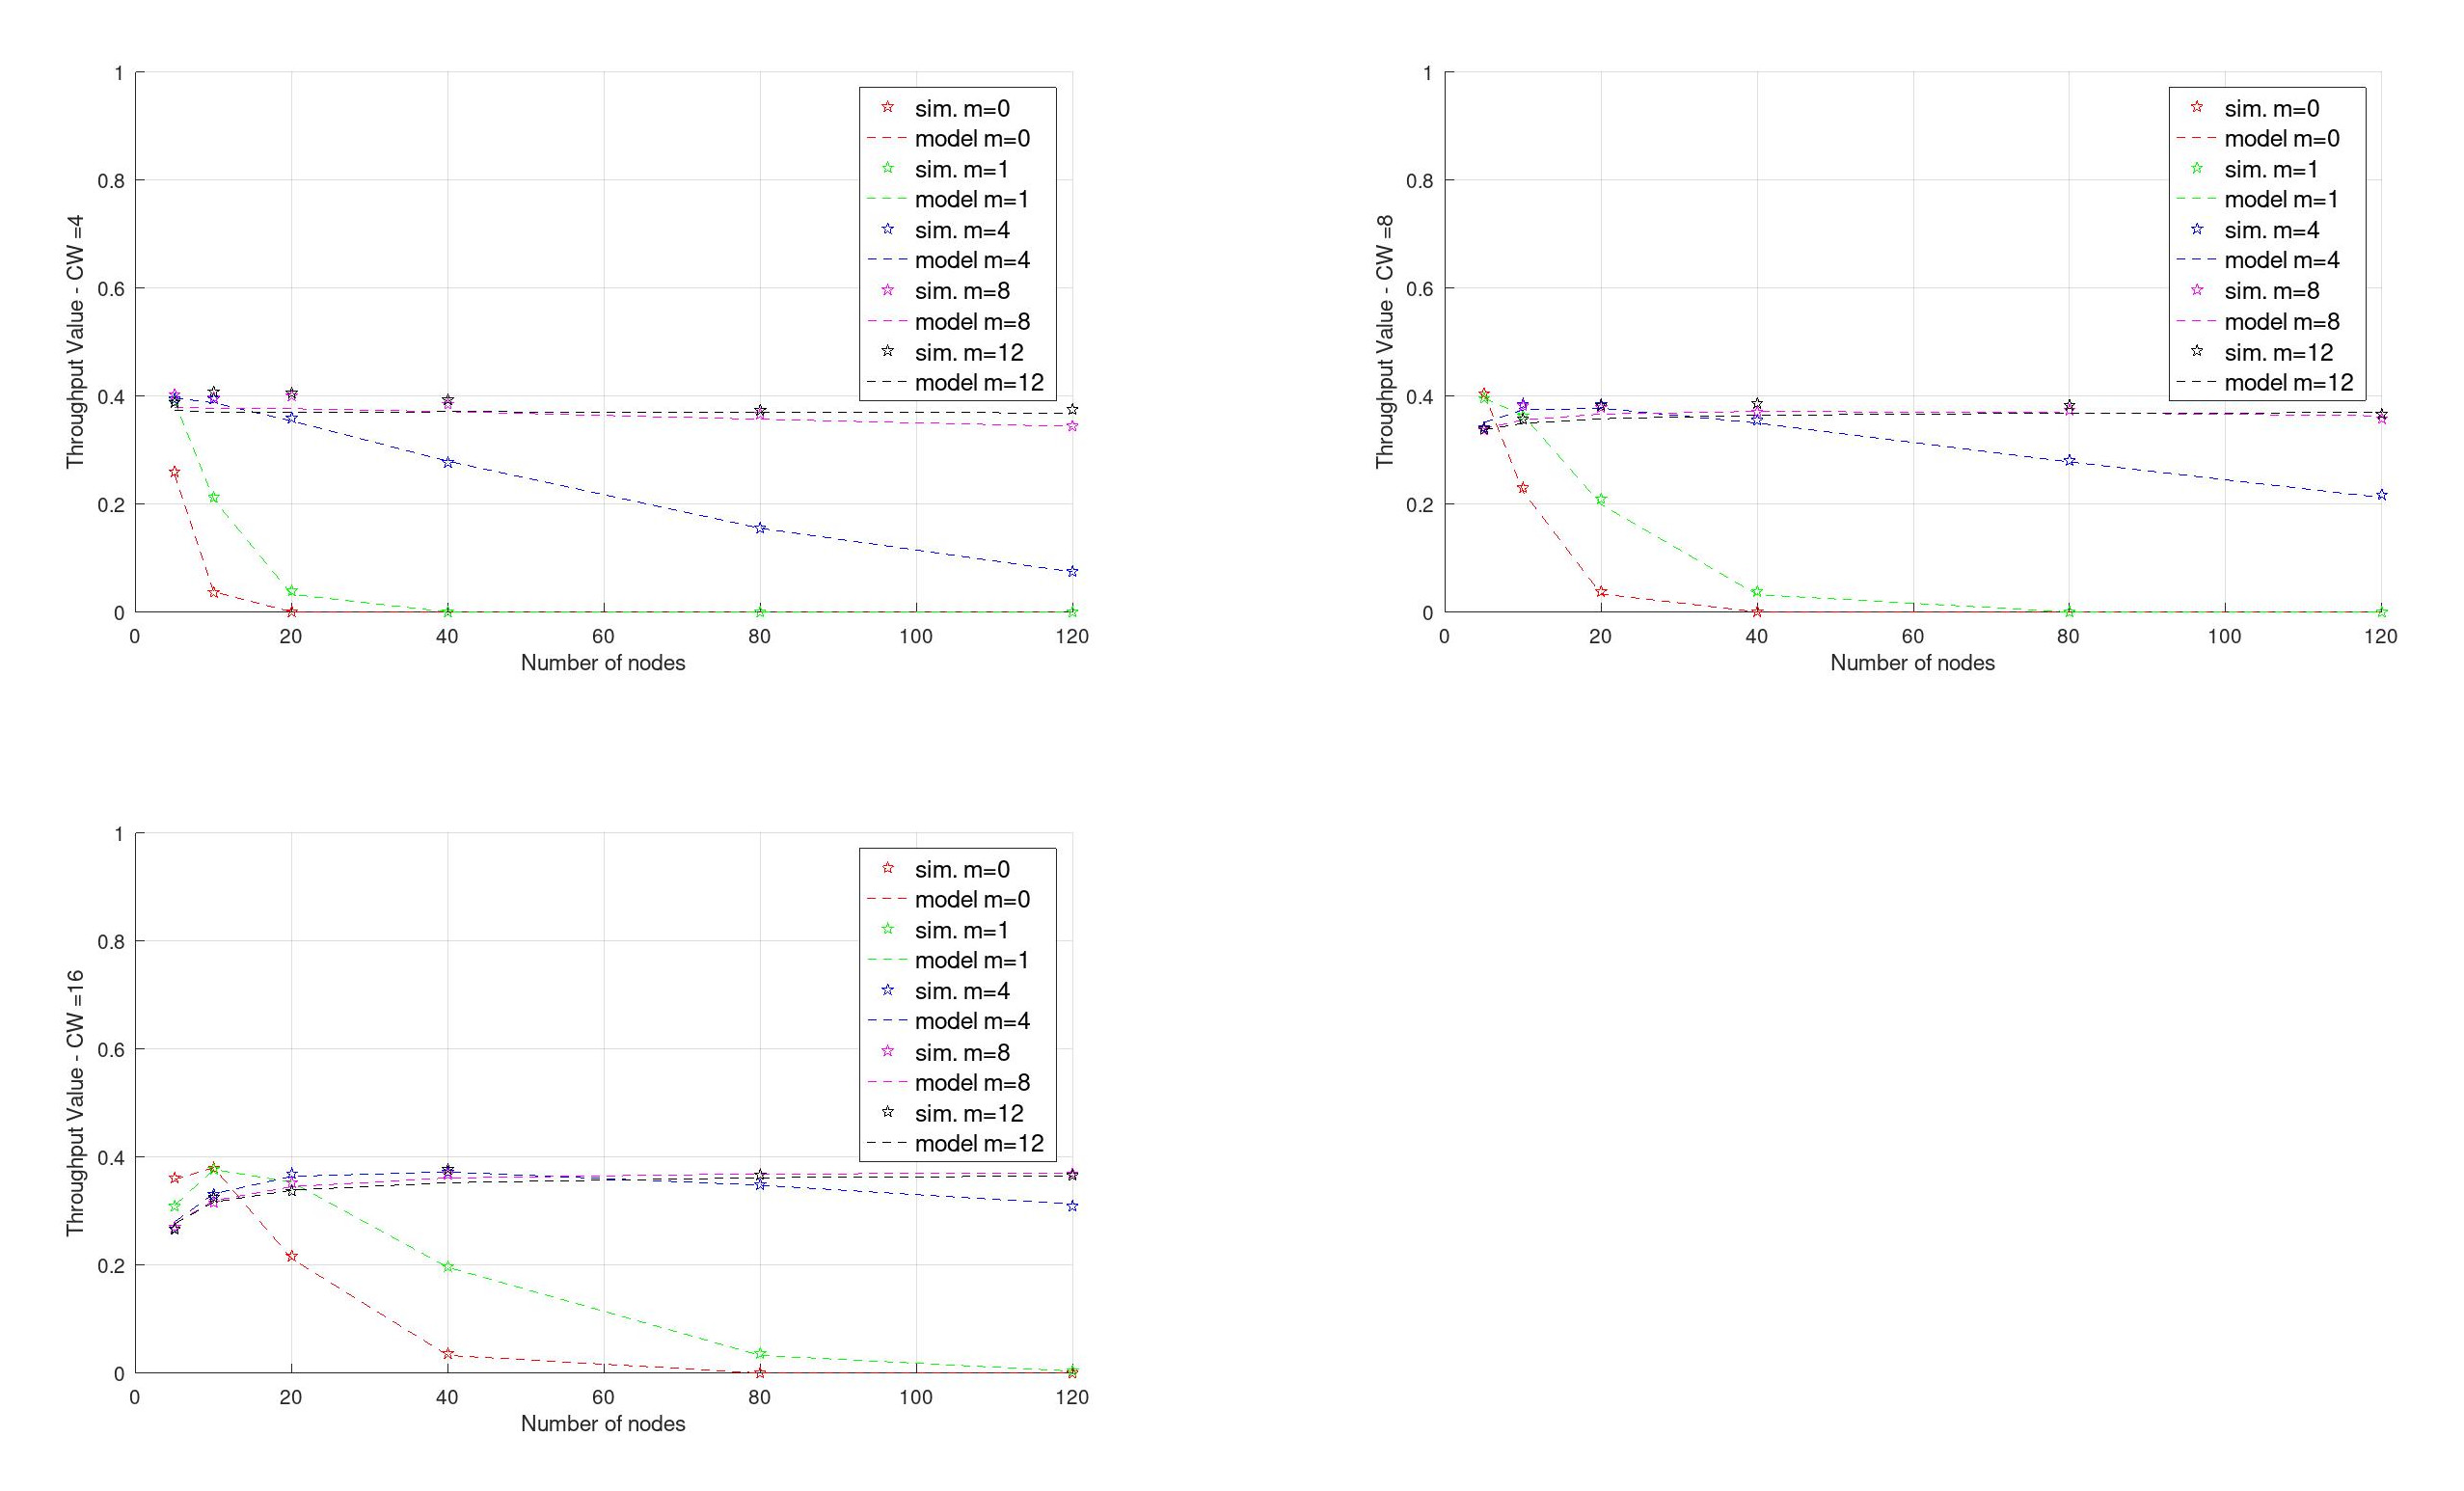
\includegraphics[scale=.18]{Images/objetivo2_2.jpeg}
    \caption{Débito para $T_{idle} = T_{succ} = T_{coll}$}
    \label{fig:objetivo2_2}
\end{figure}
\vspace{\baselineskip}

Nas Figuras \ref{fig:objetivo2_1} e \ref{fig:objetivo2_2} podemos observar os 2 casos
referidos acima. Podemos observar que, tal como no primeiro objetivo, para valores de
\textit{m} baixos (abaixo de 4), o valor de débito é bastante baixo para um número
elevado de nós. Isto muito provavelmente é causado pelo elevado número de colisões,
causadas pelo baixa janela de transmissão, que atrasam bastante todas as transmissões
futuras.
Também podemos observar no \textit{slotted} ALOHA que o valor de débito chega ao seu
máximo nos 40\%, enquanto que no IEEE 802.11 existem débitos bem acima dos 40\%
(dependendo do número de nós). Assim, podemos concluir que uma implementação com
um tempo de transmissão superior a um \textit{slot} normal traz melhores resultados que
uma implementação com \textit{slots} de igual tamanho, mesmo que isso leve a um tempo
de colisão bastante alto.